\marginnote{Beginning of structure\_intro.tex}

\subsection{Structural Variation}
\label{sec-structural}



Natural object categories such as cars and people exhibit two kinds of
variation: continuous or ``plastic'' deformations and discontinuous
structural variations. Therefore, object models which allow for both
will make vision algorithms much more powerful.  The potential for a
satisfying account of large structural variation is one of the most
intriguing possibilities of grammatical methods.

One of the simplest structural variations is occlusion: part of an
object may not be visible, usually because something between the
object and the camera is occluding it. Occlusion has been well
understood in computer vision for a long time, and models can be made
robust to it, e.g., the Hausdorff distance in \cite{hausdorff}. 

Another common way that objects exhibit structural variation is by
having \emph{optional parts}: a dog may or may not have a tail, a
person may or may not have a hat. Occlusion models are capable of
recognizing such objects with or without their optional parts, but
they do not accurately model optional parts. An optional part is a
particular subset of the object that is likely to not appear, while
occlusion allows any not-too-large subset of the model to disappear.

The usefulness of more general structural variation can be seen in
Figure \ref{fig-variation}. Here, the human eye notices a large
similarity between the two shapes $A_1$ and $A_2$, but many curve
models would see very little similarity.

\begin{figure}
  \centering
\subfloat[$A_1$]{\includegraphics[height=30mm]{images/basri_original.png}}
\subfloat[$A_2$]{\includegraphics[height=30mm]{images/basri_variation.png}}\\
\subfloat[$A_3$]{\includegraphics[height=30mm]{images/basri_variation_bad2.png}}
\subfloat[$A_4$]{\includegraphics[height=30mm]{images/basri_three.png}}
\caption{If $A_1$ is the original curve, which other curve is most
  similar to it? Figure adapted from .}
\label{fig-variation}
\end{figure}
\footnote{\cite{basri-jacobs}}

We might intuitively describe the second shape, $A_2$, as
$$ A_2 =\mbox{``Take $A_1$, snap off the right appendage, and reattach
  it beneath the left appendage.''}. \label{desc-variation}$$ 
This highlights several important points:

The description \ref{desc-variation} of $A_2$ is very short in
English, and might be even shorter in a specialized curve model
encoding. Description length is a good proxy for the conditional
probability of observing $A_2$ given that it is a distortion of $A_1$
\cite{potter-geman-bienenstock}.

Structural variation is a fundamental problem in modeling visual
objects. In the absence of a practical model of structural variation,
we must model variation as continuous deformation. Then, any model
that declares $A_1$ and $A_2$ to be similar will think that $A_3$ or
$A_4$ is even more similar to $A_1$.

Structural variation cannot be modeled without a semantically
meaningful decomposition of the original curve, like that seen in
Figure \ref{fig-variation-decompose}. Description \ref{desc-variation}
crucially relies on ``the right appendage'' making sense to the
listener. Thus, perceptually simple structural variation must respect
the perceived structure of the original curve. Contrast Figure
\ref{fig-variation} with Figure \ref{fig-badvariation}, where a
similar transformation has been applied with no regard to the
perceived structure of the original curve.

\begin{figure}[h]
\centering
\includegraphics[height=30mm]{images/basri_decomposed.png} 
\caption{The original shape from Figure \ref{fig-variation},
  decomposed into semantically meaningful parts. We argue that this
  decomposition explains why the variation in Figure
  \ref{fig-variation} is less semantically different than the
  variation in Figure \ref{fig-badvariation}. Adapted from
.}
\label{fig-variation-decompose}
\end{figure}
\footnote{\cite{basri-jacobs}}

\begin{figure}[h]
\centering
\includegraphics[height=30mm]{images/basri_original.png} 
\includegraphics[height=30mm]{images/basri_variation_bad.png} 
\caption{Two shapes which are not perceptually very similar, although
  they are related by a transformation as simple as that in Figure
  \ref{fig-variation}. The problem is that the transformation does not
  respect the perceived structure of the original. Adapted from
  .}
\label{fig-badvariation}
\end{figure}
\footnote{\cite{basri-jacobs}}

Mixture models are a class of models that do not suffer from the
continuous deformation problem of Figure \ref{fig-variation}. However,
if there are multiple independent structural variations possible, it
is unlikely that we will see every combination of each form.  Consider
the shape grammar $\GGG_n$ that generates shapes that have $n$ arms,
each of which can take either of two forms:
\begin{align*}
S&\to \underbrace{Z\dots Z}\\
&\phantom{\to Z ..}n\\
Z &\to A\\
Z &\to B,
\end{align*}
where $A$ is pointy and $B$ is rectangular. We show four shapes
possible under this grammar in Figure \ref{fig-narms}. 
\marginnote{Change these to outline instead of solid shapes!}
\begin{figure}[h]
\centering
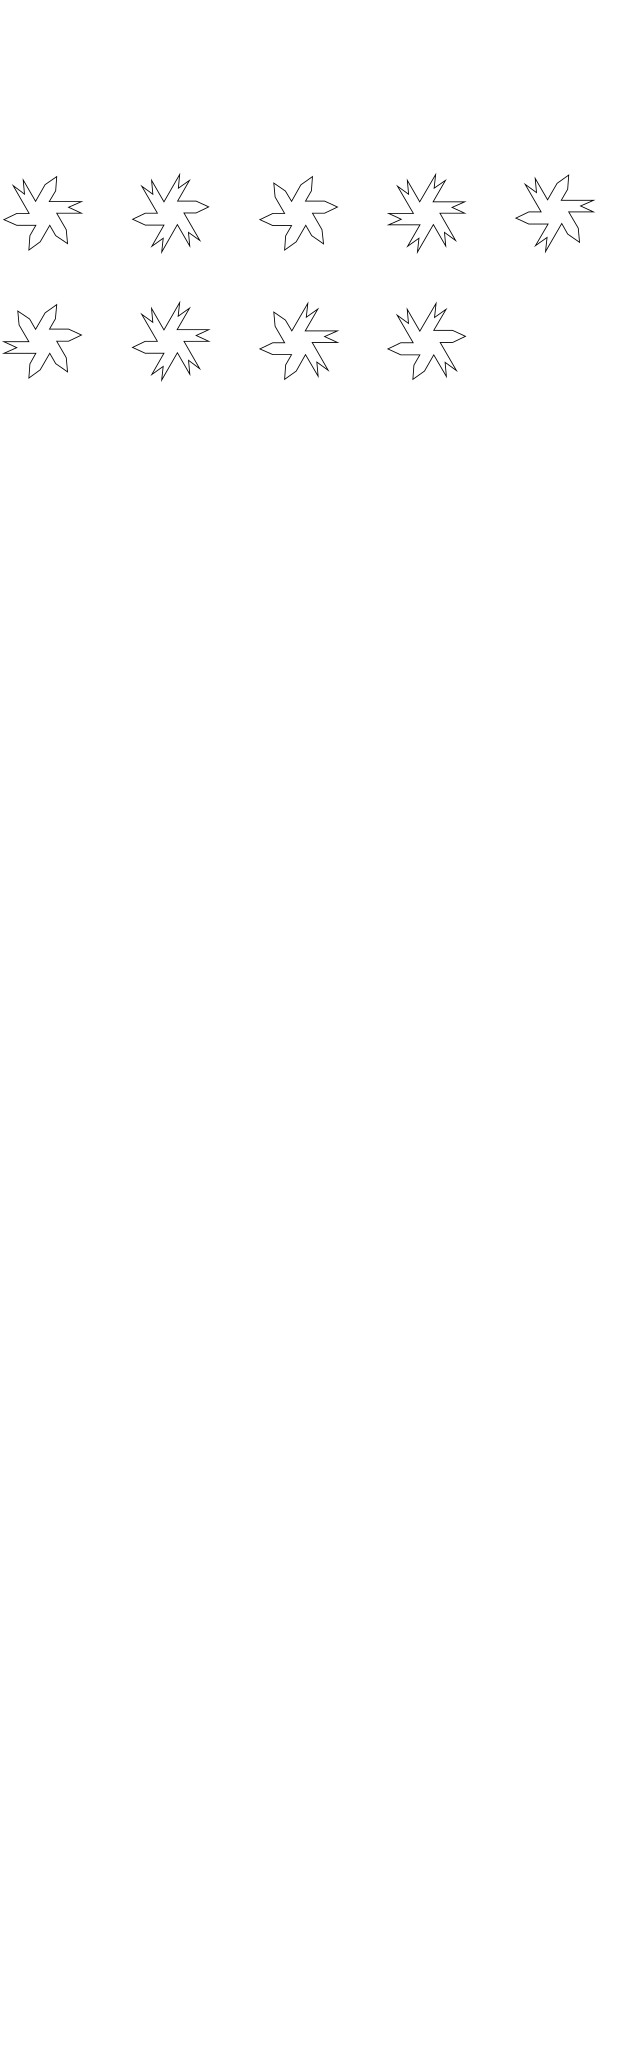
\includegraphics[height=30mm]{images/narms.png} 
\caption{Four shapes from $\GGG_8$.}
\label{fig-narms}
\end{figure}
A classic mixture model will not be able to generalize in this
scenario without exponentially many training examples, since there
are $2^n$ possible shapes. If we instead have mixture models at the
level of individual structural variations, then our model is a
grammatical model in the style of Section \ref{sec-grammar-examples}.

\marginnote{End of structure\_intro.tex}